\documentclass[border=2pt]{standalone}
\usepackage[T1]{fontenc}\usepackage{helvet}\renewcommand{\familydefault}{\sfdefault}
\usepackage[helvet]{sfmath}
\usepackage{tikz}\usetikzlibrary{arrows.meta,shapes.geometric,calc}
\definecolor{dg}{HTML}{1E5A3C}\definecolor{lg}{HTML}{EEF5F0}\definecolor{dr}{HTML}{A33A3A}\definecolor{lr}{HTML}{FBEFEF}
\begin{document}
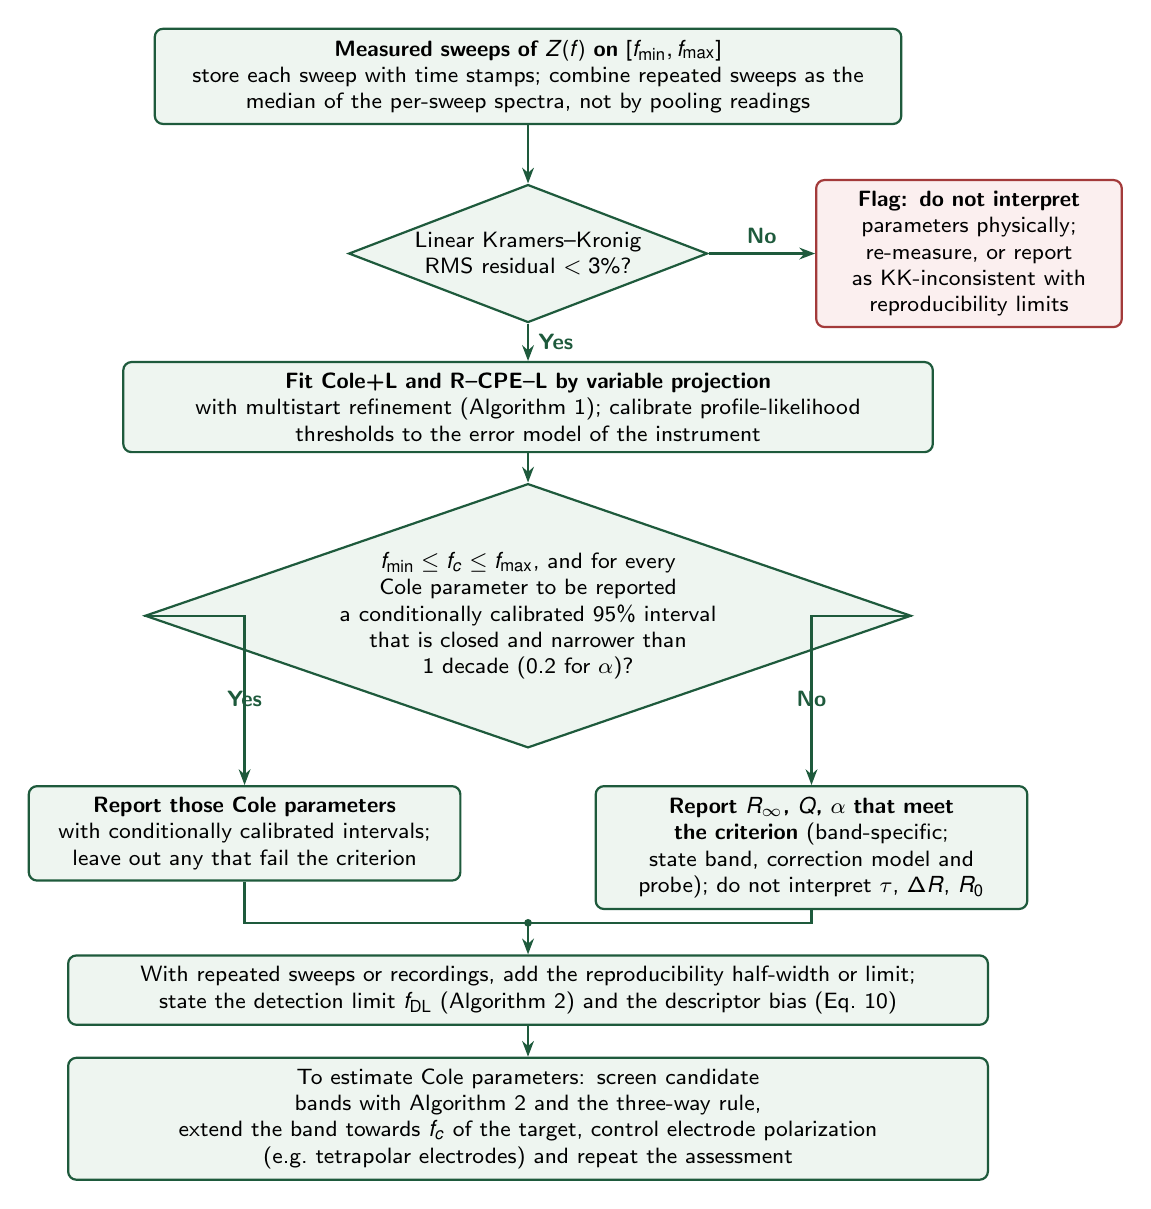
\begin{tikzpicture}[font=\footnotesize,
 box/.style={draw=dg,fill=lg,rounded corners=3pt,line width=0.8pt,align=center,inner sep=4pt},
 dec/.style={diamond,draw=dg,fill=lg,line width=0.8pt,align=center,inner sep=1pt},
 bad/.style={draw=dr,fill=lr,rounded corners=3pt,line width=0.8pt,align=center,inner sep=4pt,text width=3.6cm},
 arr/.style={-{Stealth[length=2mm]},line width=0.8pt,dg},
 lab/.style={font=\footnotesize\bfseries,text=dg}]
\node[box,text width=9.2cm] (m) at (0,0) {\textbf{Measured sweeps of $Z(f)$ on $[f_{\min},f_{\max}]$}\\store each sweep with time stamps; combine repeated sweeps as the\\median of the per-sweep spectra, not by pooling readings};
\node[dec,aspect=2.6] (kk) at (0,-2.25) {Linear Kramers--Kronig\\RMS residual $<3\%$?};
\node[bad] (flag) at (5.6,-2.25) {\textbf{Flag: do not interpret}\\parameters physically; re-measure, or report as KK-inconsistent with reproducibility limits};
\node[box,text width=10cm] (fit) at (0,-4.2) {\textbf{Fit Cole+L and R--CPE--L by variable projection}\\with multistart refinement (Algorithm~1); calibrate profile-likelihood\\thresholds to the error model of the instrument};
\node[dec,aspect=2.9] (id) at (0,-6.85) {$f_{\min}\le f_c\le f_{\max}$, and for every\\Cole parameter to be reported\\a conditionally calibrated 95\% interval\\that is closed and narrower than\\1 decade (0.2 for $\alpha$)?};
\node[box,text width=5.2cm,anchor=north] (yes) at (-3.6,-9.0) {\textbf{Report those Cole parameters}\\with conditionally calibrated intervals;\\leave out any that fail the criterion};
\node[box,text width=5.2cm,anchor=north] (no) at (3.6,-9.0) {\textbf{Report $R_{\infty}$, $Q$, $\alpha$ that meet}\\\textbf{the criterion} (band-specific; state band, correction model and probe); do not interpret $\tau$, $\Delta R$, $R_0$};
\node[box,text width=11.4cm,anchor=north] (rep) at (0,-11.15) {With repeated sweeps or recordings, add the reproducibility half-width or limit;\\state the detection limit $f_{\mathrm{DL}}$ (Algorithm~2) and the descriptor bias (Eq.~10)};
\node[box,text width=11.4cm,anchor=north] (ext) at (0,-12.45) {To estimate Cole parameters: screen candidate bands with Algorithm~2 and the three-way rule,\\extend the band towards $f_c$ of the target, control electrode polarization\\(e.g.\ tetrapolar electrodes) and repeat the assessment};
\draw[arr] (m) -- (kk); \draw[arr] (kk) -- node[lab,above]{No} (flag);
\draw[arr] (kk) -- node[lab,right]{Yes} (fit); \draw[arr] (fit) -- (id);
\draw[arr] (id.west) -| node[lab,above,pos=0.8]{Yes} (yes.north);
\draw[arr] (id.east) -| node[lab,above,pos=0.8]{No} (no.north);
\coordinate (j) at (0,-10.75);
\draw[line width=0.8pt,dg] (yes.south) |- (j) -| (no.south); \fill[dg] (j) circle (1.4pt);
\draw[arr] (j) -- (rep); \draw[arr] (rep) -- (ext);
\end{tikzpicture}
\end{document}
